\documentclass{article}

% Language setting
\usepackage[polish]{babel}

% Set page size and margins
% Replace `letterpaper' with `a4paper' for UK/EU standard size
\usepackage[letterpaper,top=2cm,bottom=2cm,left=3cm,right=3cm,marginparwidth=1.75cm]{geometry}

% Useful packages
\usepackage{amsmath}
\usepackage{graphicx}
\usepackage[T1]{fontenc}
\usepackage[colorlinks=true, allcolors=blue]{hyperref}
\usepackage{lipsum}
\usepackage{multicol}
\usepackage{tikz,tcolorbox}
\usepackage{float}

\title{Metoda klasyfikacji cukierków na podstawie ich opakowania}
\author{Aleksander Golus, Bartosz Chadryś, Jakub Miśko, Igor Joński}

\begin{document}
\maketitle

\newpage

\definecolor{my-red-light}{RGB}{254, 218, 212}
\definecolor{my-red-dark}{RGB}{220, 97, 85}
\definecolor{my-orange-light}{RGB}{252, 236, 189}
\definecolor{my-orange-dark}{RGB}{247, 167, 9}
\definecolor{my-pink-light}{RGB}{252, 218, 229}
\definecolor{my-pink-dark}{RGB}{247, 132, 168}
\definecolor{my-green}{RGB}{141, 189, 16}

\section{Wstęp}
\label{Wstęp}
W projekcie opracowano metodę, która pozwala rozpoznawać typy cukierków na podstawie ich kolorowych opakowań oraz monitorować ich ilości na taśmie produkcyjnej.

Jednym z podobnych rozwiązań w tej branży (spożywczej) jest rozpoznawanie rodzajów bułek oraz ich kształtów tak jak zostało to przedstawione w artykule \cite{virtuslab}. W przypadku tematu, jakim są cukierki, można znaleźć zastosowania w pomocy rozróżniania rodzaju cukierka w bombonierce \cite{chocolates}. Innym przypadkiem użycia detekcji obiektów na podstawie ich opakowania może być również innowacyjna metoda rozpoznawania produktów w automatach sprzedających \cite{vending}.

Podobne metody znajdują również zastosowania w detekcji obiektów przenoszonych przenośnikami taśmowymi. Przykładowo, w artykule \cite{coalForeign} przedstawiono metodę detekcji obcych obiektów wystepujących na przenośniku taśmowym w kopalni węgla.

Metoda, którą opracowano w tym projekcie, może znaleźć zastosowanie w przemyśle spożywczym w automatyzacji procesów pakowania oraz kontroli jakości. Zapewnia ona selekcję produktów oraz może przyczynić się do usprawnienia procesów magazynowania i dystrybucji.

\section{Materiały i metody}
\label{Materiały i metody}
\subsection{Materiały badawcze}
\label{Materiały badawcze}
Materiałami badawczymi są konkretne rodzaje cukierków o kolorowych opakowaniach - cukierki marki Mamba oraz Turbo. Zostały one wybrane ze względu na to, że posiadają bardzo podobny rozmiar.

Wykorzystane cukierki dzielimy na 4 typy kolorów, z czego różowy, czerwony oraz pomarańczowy to cukierki marki Mamba, natomiast zielony - marki Turbo.

\begin{figure}[H]
    \centering
    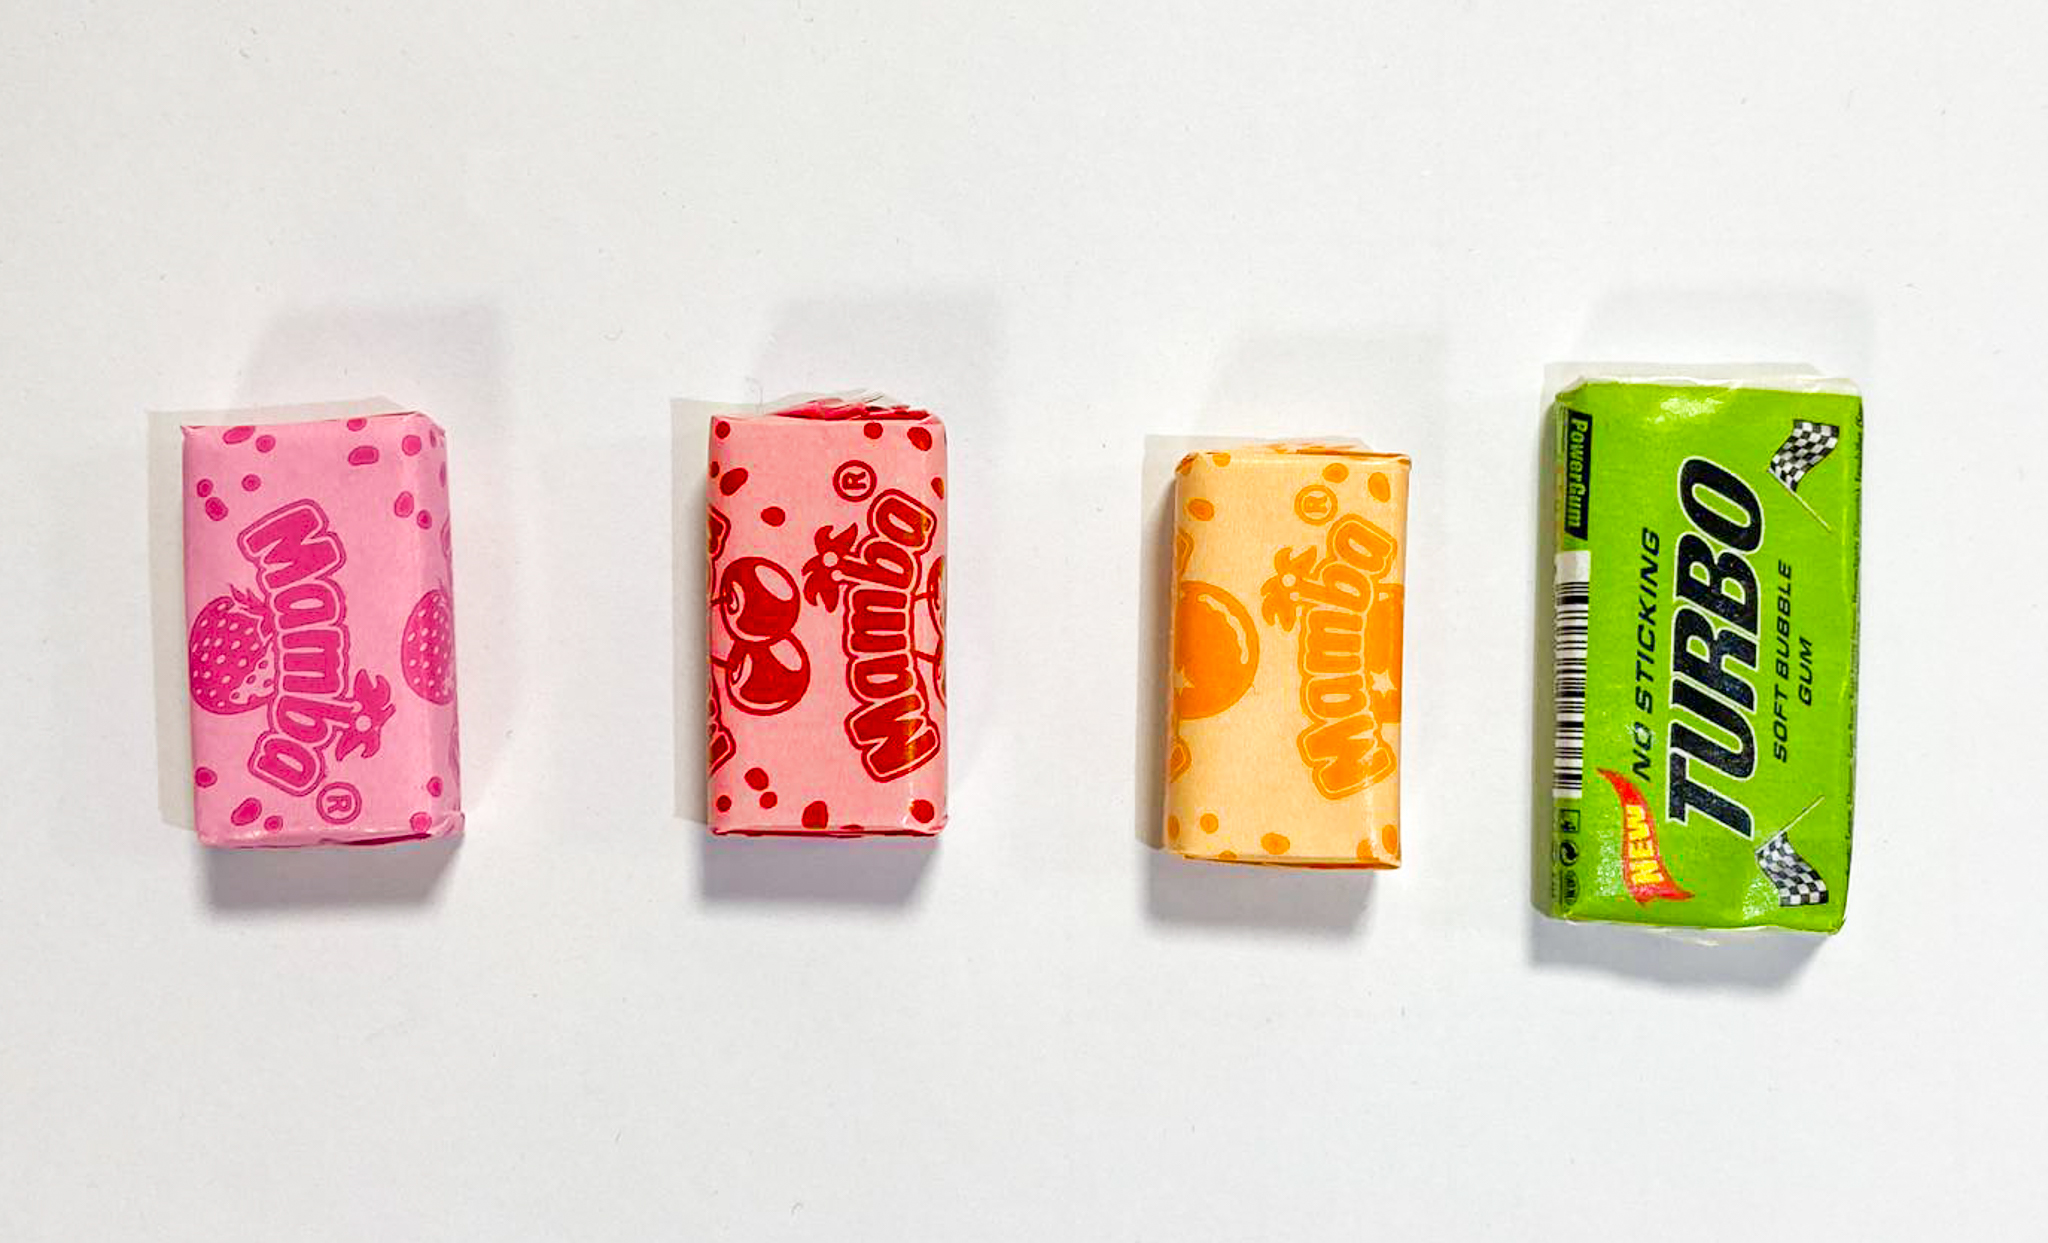
\includegraphics[width=\linewidth]{candies.jpg}
    \caption{Cukierki wykorzystane w projekcie}
\end{figure}


\subsection{Przedziały kolorów rozpoznawalnych cukierków}

Kolory cukierków w określonym oświetleniu, omówionym w sekcji \ref{Układ pomiarowy}, powinny zawierać się w następujących zakresach, by zostaly poprawnie zidentyfikowane:

\begin{table}[H]
    \label{tab:tab1}
    \centering
    \begin{tabular}{ |c|c|c|c| }
     \hline
     Kolor & Dolna granica & Górna granica \\
     \hline
     Różowy & \#32282f & \#ff0000 \\
     \hline
     Czerwony & \#645050 & \#ff7a37 \\
     \hline
     Pomarańczowy & \#644b3d & \#ffd500 \\
     \hline
     Zielony & \#323222 & \#00ff00 \\
     \hline
    \end{tabular}
    \caption{Przedziały barw, w których musi znaleźć się kolor opakowania cukierka by został zidentyfikowany.}
\end{table}

\subsection{Układ pomiarowy}
\label{Układ pomiarowy}

\begin{figure}[H]
    \centering
    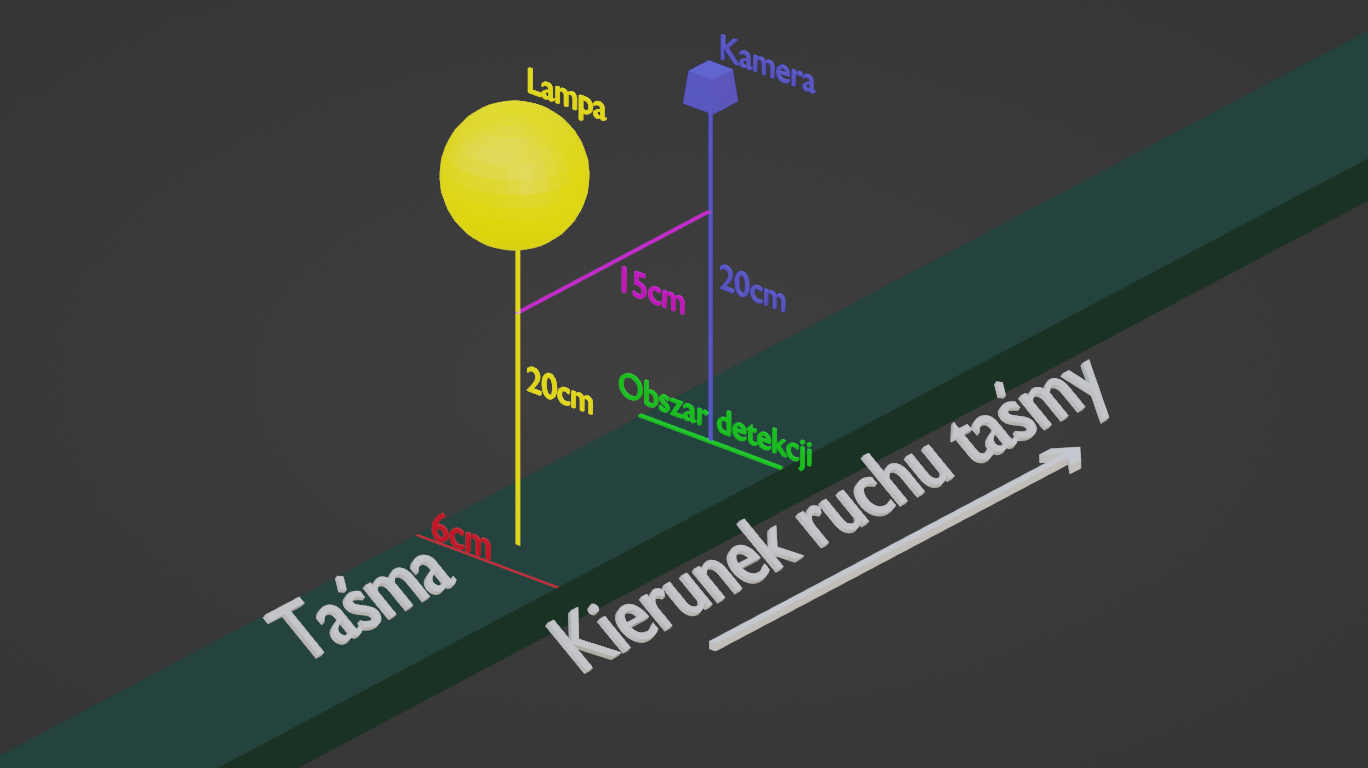
\includegraphics[width=\linewidth]{ukladPomiarowy.png}
    \caption{Układ pomiarowy}
    \label{fig:ukladPomiarowy}
\end{figure}

Układ pomiarowy, przedstawiony na rysunku \ref{fig:ukladPomiarowy}, składa się z ciemnozielonej taśmy produkcyjnej napędzanej silnikiem elektrycznym o stałej prędkości, kamery o rozdzielczości 1920x1080 pikseli nagrywającej w 30 klatkach na sekundę oraz lampy LED naświetlającej taśmę z góry. Ciemnozielony kolor taśmy został wybrany tak, aby nie zawierał się w przedziałach barw cukierków w tabeli \ref{tab:tab1}.

Taśma produkcyjna, o szerokości 6cm, przesuwa umieszczone na niej cukierki ze stałą prędkością 3cm/s. Do oświetlenia cukierków znajdujących się na taśmie została użyta lampa ledowa o mocy 10W i temperaturze 3500K, umieszczona na wysokości 20cm, oddalona od kamery o 15cm w płaszczyźnie poziomej. Kamera została ustawiona 20cm nad taśmą, rejestrując przy tym całą szerokość taśmy.

Układ pomiarowy składa się również z obszaru detekcji, czyli miejsca, w którym zliczane są typy cukierków. Obszar posiada wymiary 3mm x 6cm. Jego szerokość jest równa szerokości taśmy, natomiast długość została dobrana tak, aby każdy cukierek przynajmniej raz się w nim znalazł.

\subsection{Metoda pomiarowa}
\label{Metoda pomiarowa}
\subsubsection{Idea}
\label{Idea}

Ideą metody pomiarowej jest zliczanie cukierków umieszczonych na taśmie produkcyjnej bazując na kolorze opakowania cukierka. Przypadki użycia metody pomiarowej to między innymi:

\begin{itemize}
    \item Weryfikacja ilości cukierków w partii - czy ilość zliczonych cukierków jest zgodna z ustaloną ilością w danej partii.
    \item Weryfikacja różnorodności cukierków - czy zliczone cukierki na taśmie są wystarczająco zróżnicowane.
\end{itemize}

\subsubsection{Sposób pomiaru}
\label{Sposób pomiaru}

\begin{figure}[H]
    \centering
    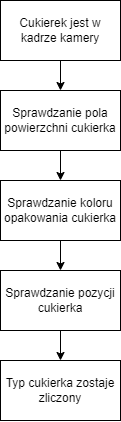
\includegraphics[height=8cm]{diagramMetody.png}
    \caption{Diagram metody pomiarowej}
    \label{fig:diagramMetody}
\end{figure}

Metoda, przedstawiona na ryusnku \ref{fig:diagramMetody}, by zidentyfikować i zliczyć typ danego cukierka wykonuje następujące kroki:
\begin{enumerate}
    \item Sprawdzany zostaje kolor opakowania cukierka, który musi zawierać się w jednym z określonych w tabeli \ref{tab:tab1} przedziałach. By to określić:
    \begin{itemize}
        \item Dla każdego z 4 przedziałów barw, tworzona jest maska, na której cukierki badanego koloru są reprezentowane jako białe obszary, a tło jako czarne.
        \item Do utworzenia masek wykorzystana zostaje funkcja \verb|cv2.inRange()|\cite{inRange}, przyjmująca jako argumenty: klatkę aktualnie analizowanego obrazu w przestrzeni barw HSV, dolną oraz górną granicę danego przedziału barw.
        \item Zwrócone zostają łącznie 4 maski, po jednej dla każdego przedziału barw. \textbf{Wszystkie kolejne kroki są wykonywane dla każdej z 4 otrzymanych masek osobno}.
    \end{itemize}
    \item Sprawdzane jest pole powierzchni identyfikowanego cukierka, które musi być większe niż minimalne założone pole (30000px):
    \begin{itemize}
        \item Dla każdej z otrzymanych masek wyznaczamy kontury znalezionych obiektów.
        \item Do znalezienia konturów wykorzystana zostaje funkcja \verb|cv2.findContours()|\cite{findContours}, przyjmująca jako argumenty: obraz binarny (jedna z 4 wcześniej otrzymanych masek), tryb konturów (użyliśmy \verb|RETR_EXTERNAL|\cite{retrExternal}, który zwraca nam tylko zewnętrzne kontury, a wszystkie zagnieżdżone wewnętrzne kontury są pomijane) oraz metoda aproksymacji konturów (skorzystaliśmy z \verb|CHAIN_APPROX_SIMPLE|\cite{chainApproxSimble}, która kompresuje informacje o konturze do 4 punktów wyznaczających narożniki konturu, co jest dla nas wystarczającą informacją).
        \item Dla wszystkich otrzymanych konturów, obliczane jest zaznaczone przez nie pole powierzchni. Obiekty, których pole powierzchni jest większe niż minimalne założone pole, są wykorzystywane w kolejnym kroku.
    \end{itemize}
    \item Sprawdzana jest pozycja konturu cukierka. Do analizy pozycji konturów wszystkich cukierków wykorzystaliśmy listę obserwowanych konturów, która jest aktualizowana w każdej klatce:
    \begin{itemize}
        \item Dla każdego konturu sprawdzana jest jego pozycja (środek ciężkości) na obrazie.
        \item Jeżeli w liście obserwowanych konturów istnieje kontur, którego pozycja, względem aktualnie analizowanego konturu, wzdłuż i w poprzek ruchu taśmy nie zmieniła się (z dokładnością do 40px), to kontur z listy zostaje zidentyfikowany jako ten aktualnie analizowany, a jego pozycja zostaje zaktualizowana. Jeżeli nie istnieje taki kontur, to aktualnie analizowany kontur zostaje dodany do listy obserwowanych konturów.
        \item Jeżeli aktualnie analizowany kontur znajduje się w obszarze detekcji, to ilość rozpoznanego rodzaju cukierka jest zwiększana, a sam kontur otrzymuje flagę, że został już rozpoznany.
    \end{itemize}
\end{enumerate}

\section{Wyniki i dyskusja}
\label{Wyniki i dyskusja}
Skuteczność działania metody została przetestowana na wcześniej przygotowanym nagraniu taśmy produkcyjnej z umieszczonymi na niej cukierkami. Nagranie przedstawia przykładowe działanie metody.
\subsection{Wyniki}
Analizując rezultaty otrzymaliśmy następujące wyniki:

\begin{figure}[H]
    \centering
    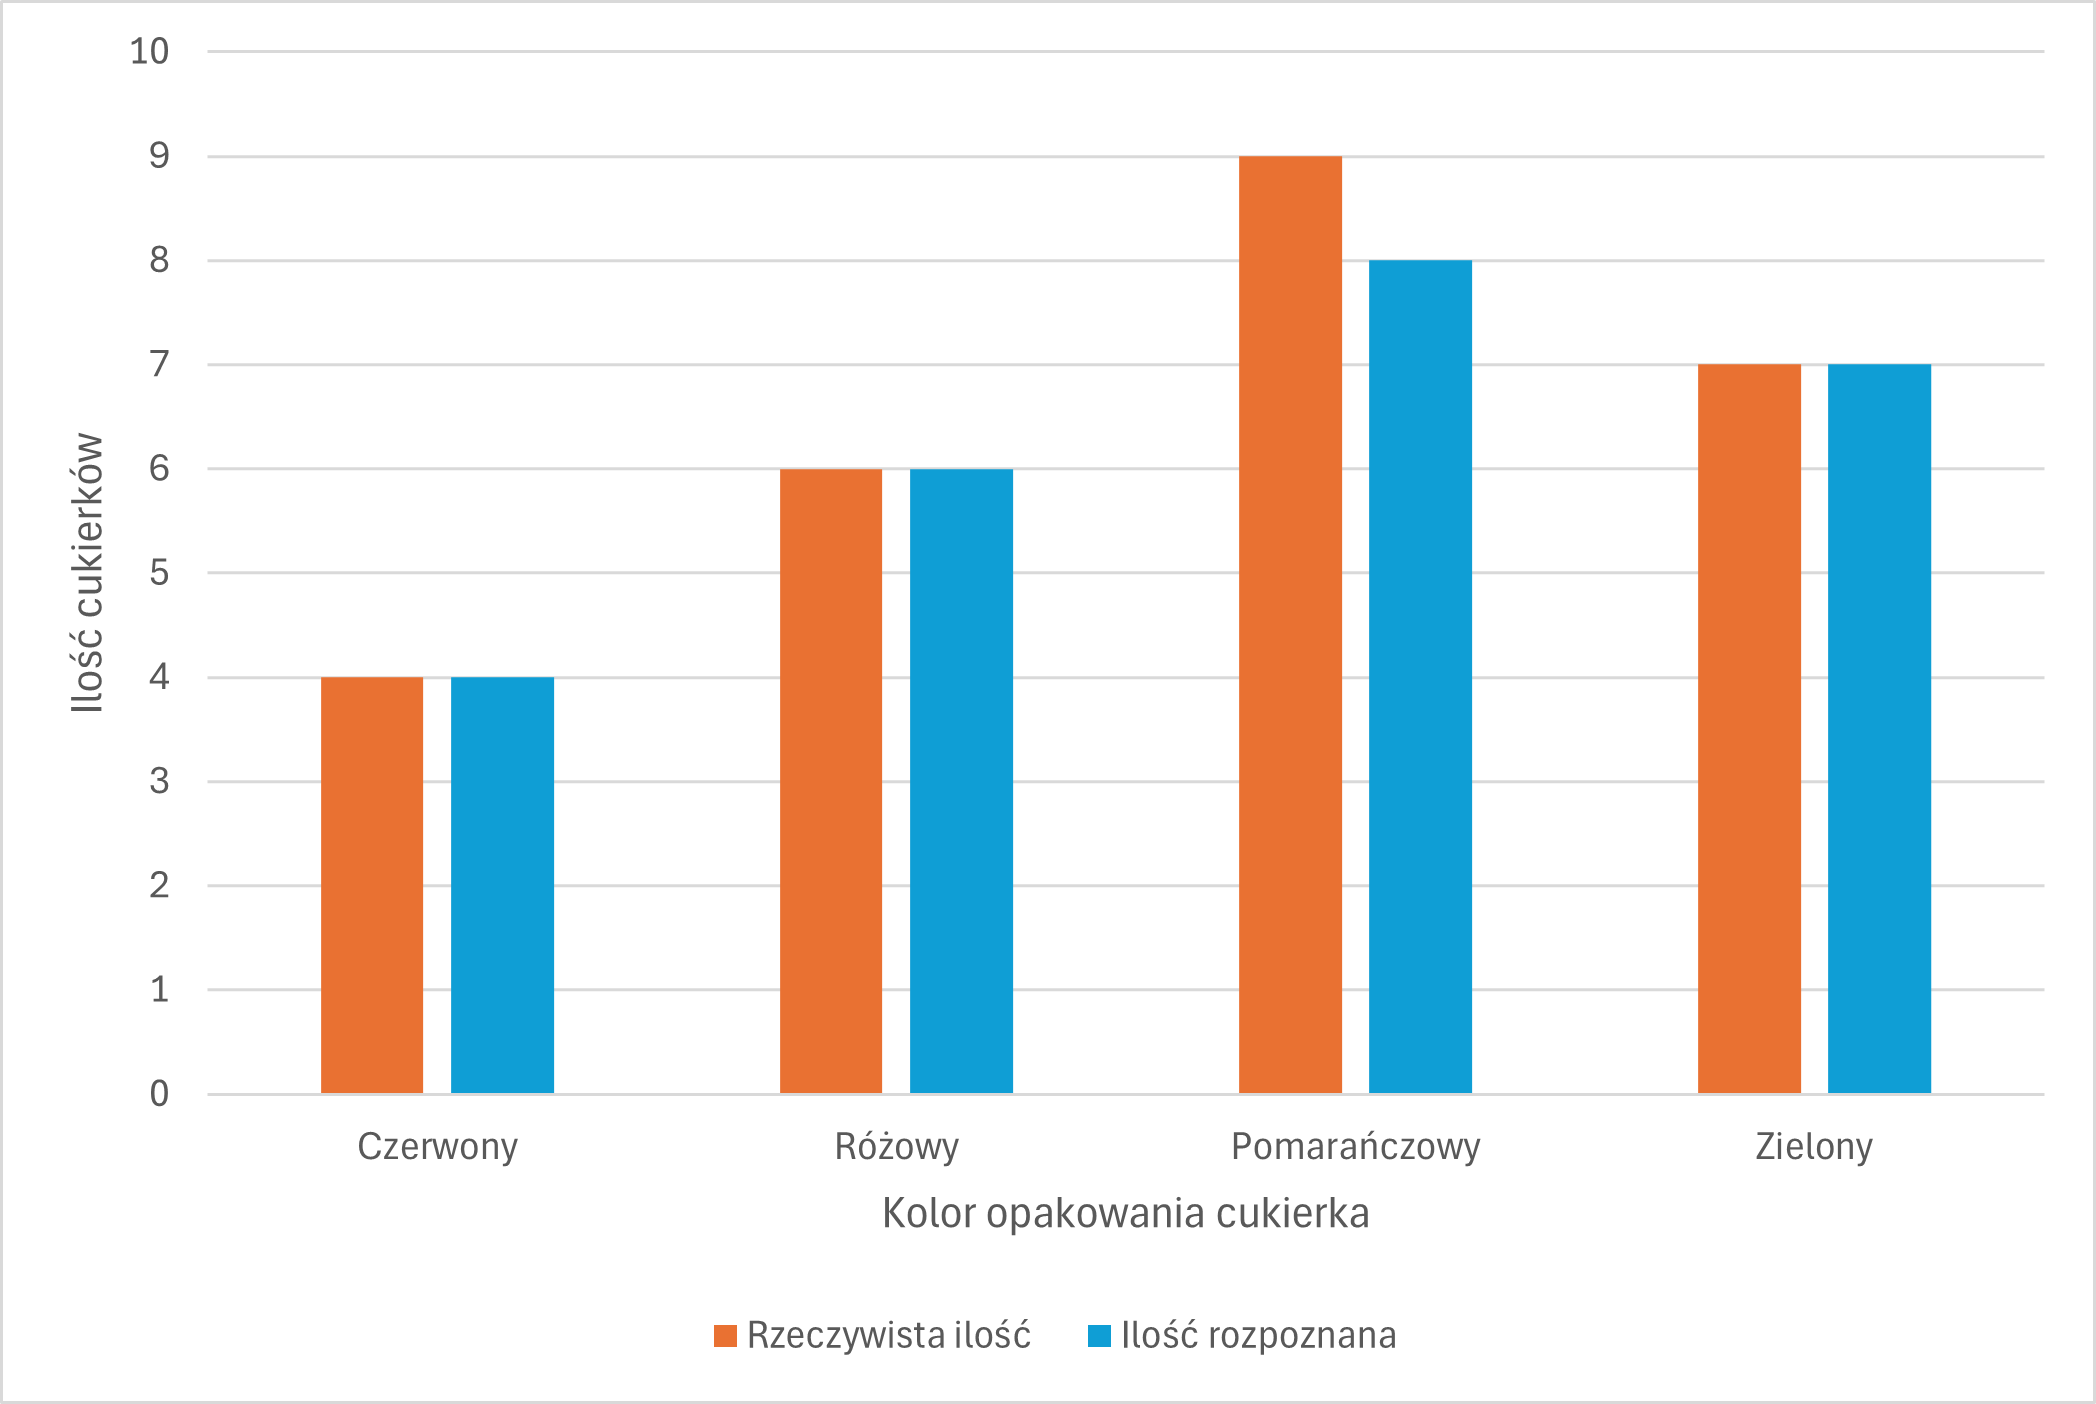
\includegraphics[width=\linewidth]{wykresSkutecznosci}
    \caption{Wykres rezultatów dla przykładowego działania metody}
    \label{fig:wykresSkutecznosci}
\end{figure}

Analizując rysunek \ref{fig:wykresSkutecznosci} można zauważyć, że metoda klasyfikacji cukierków nie zliczyła wszystkich cukierków, które zostały umieszczone na taśmie.

W celu zbadania przyczyny tego zjawiska, przeanalizowaliśmy nagranie, na którym została uruchomiona metoda. W wyniku analizy, zauważyliśmy, że metoda nie zliczyła poprawnie cukierków o tym samym kolorze opakowania, które znajdowały się bezpośrednio obok siebie - w tym przypadku, metoda zliczyła jeden cukierek, a drugi pominęła.

\subsection{Przykład opisanego błędu}
\label{Przykład opisanego błędu}
W celu potwierdzenia przyczyny błędu, przeprowadziliśmy dodatkowy test, który polegał na umieszczeniu na taśmie dwóch cukierków tego samego koloru opakowania obok siebie. Wykorzystaliśmy do tego trzy pary cukierków, czerwonych, różowych oraz pomarańczowych. Rysunek \ref{fig:wykresBledu} przedstawia wyniki testu.

\begin{figure}[H]
    \centering
    \label{fig:wykresBledu}
    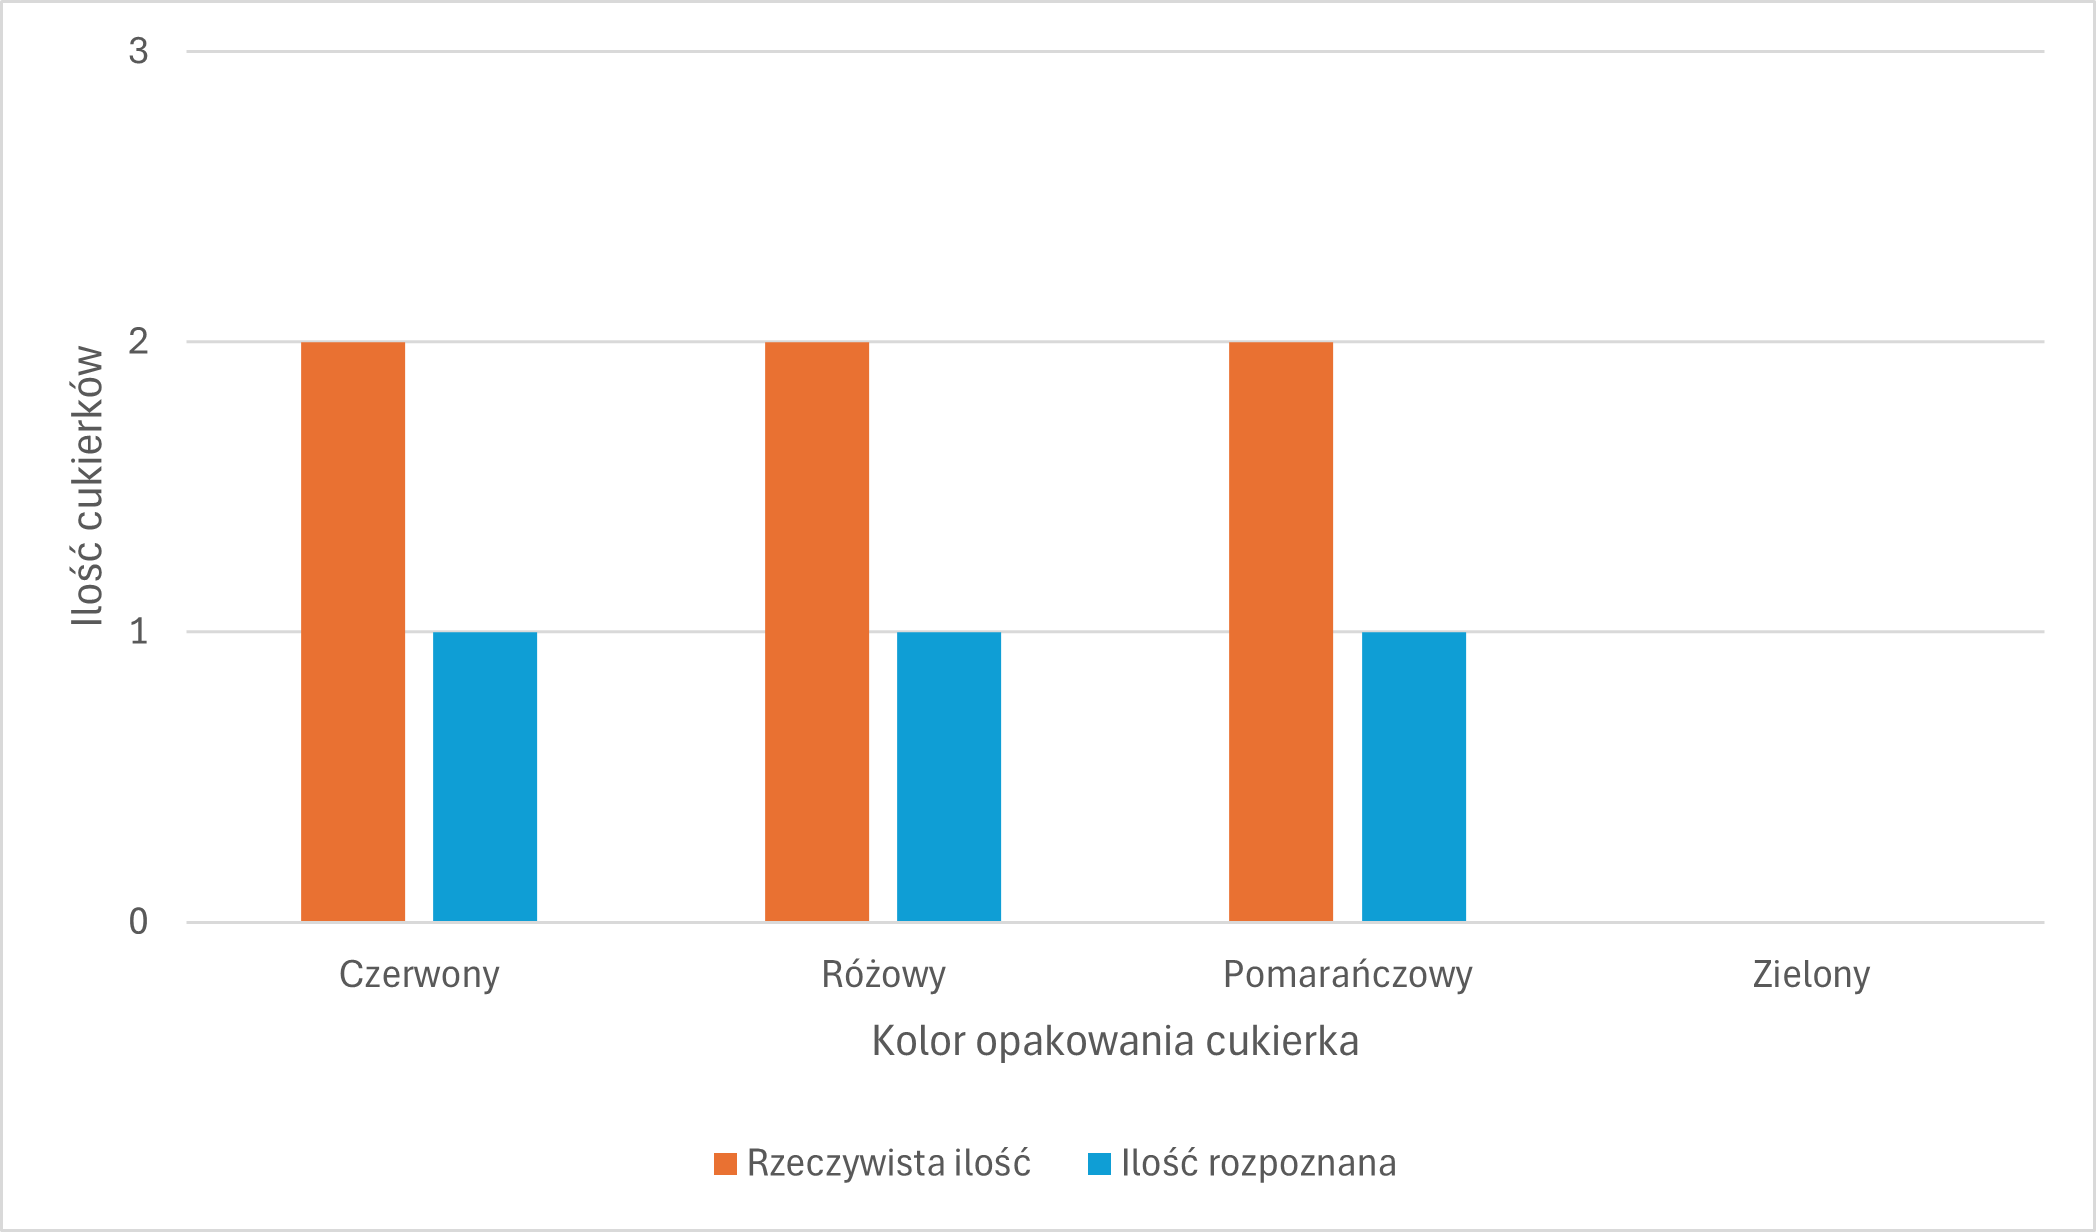
\includegraphics{wykresBledu}
    \caption{Wyniki testu potwierdzającego przyczynę błędu}
\end{figure}

Analizując rysunek \ref{fig:wykresBledu} można zauważyć, że metoda zliczyła poprawnie tylko jeden cukierek z każdej pary, co potwierdza naszą hipotezę, że metoda nie zliczy cukierków o tym samym kolorze opakowania, które znajdują się bezpośrednio obok siebie.

\begin{center}
\begin{figure}[H]
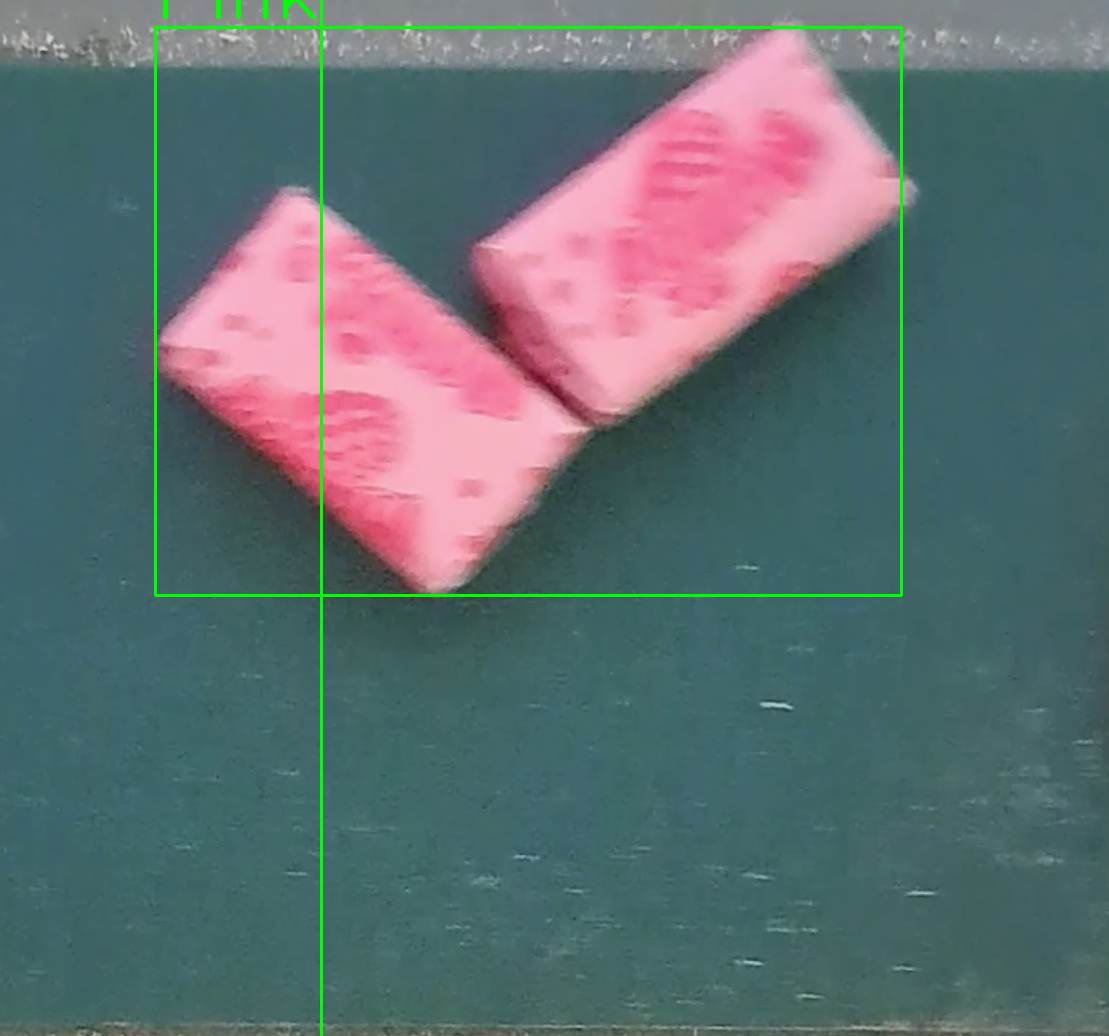
\includegraphics[height=5cm]{pink.png}
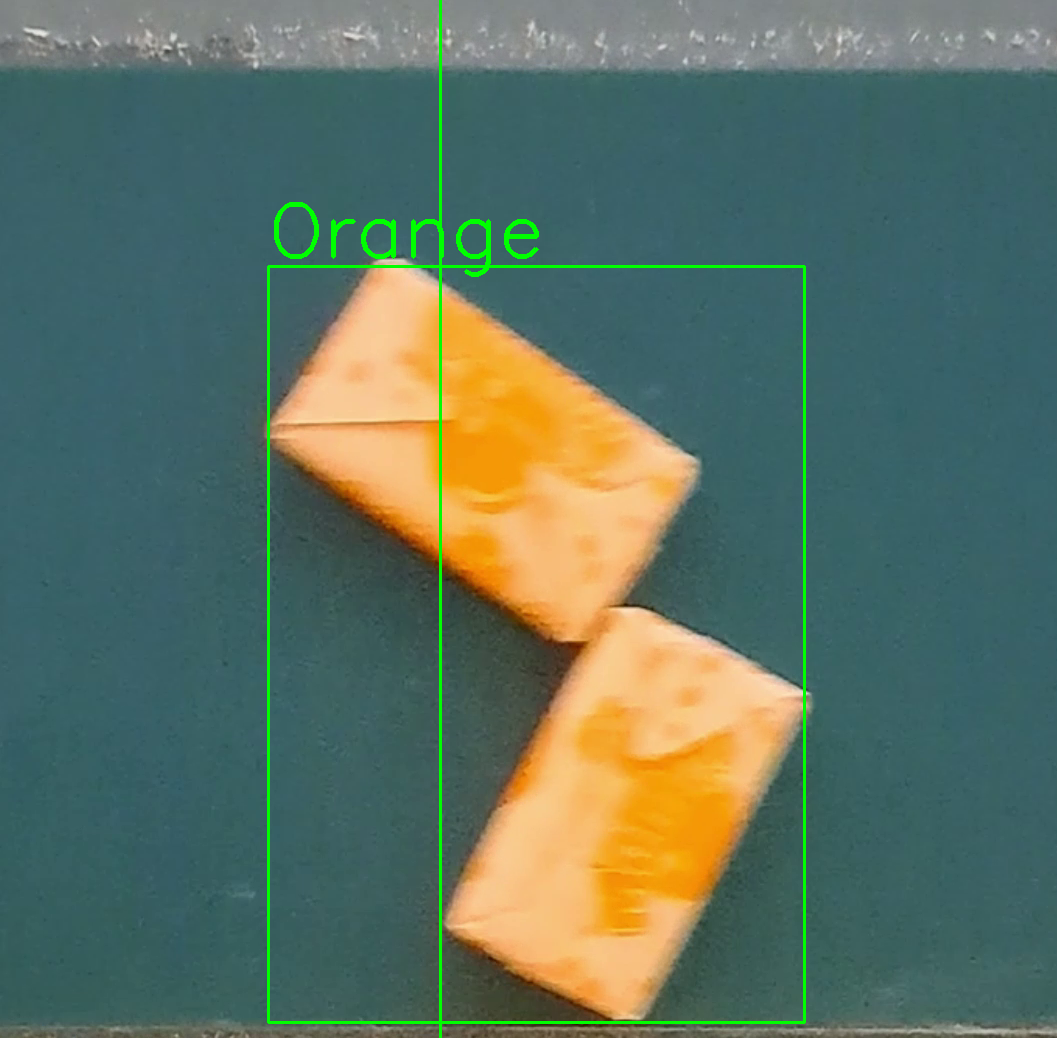
\includegraphics[height=5cm]{orange.png}
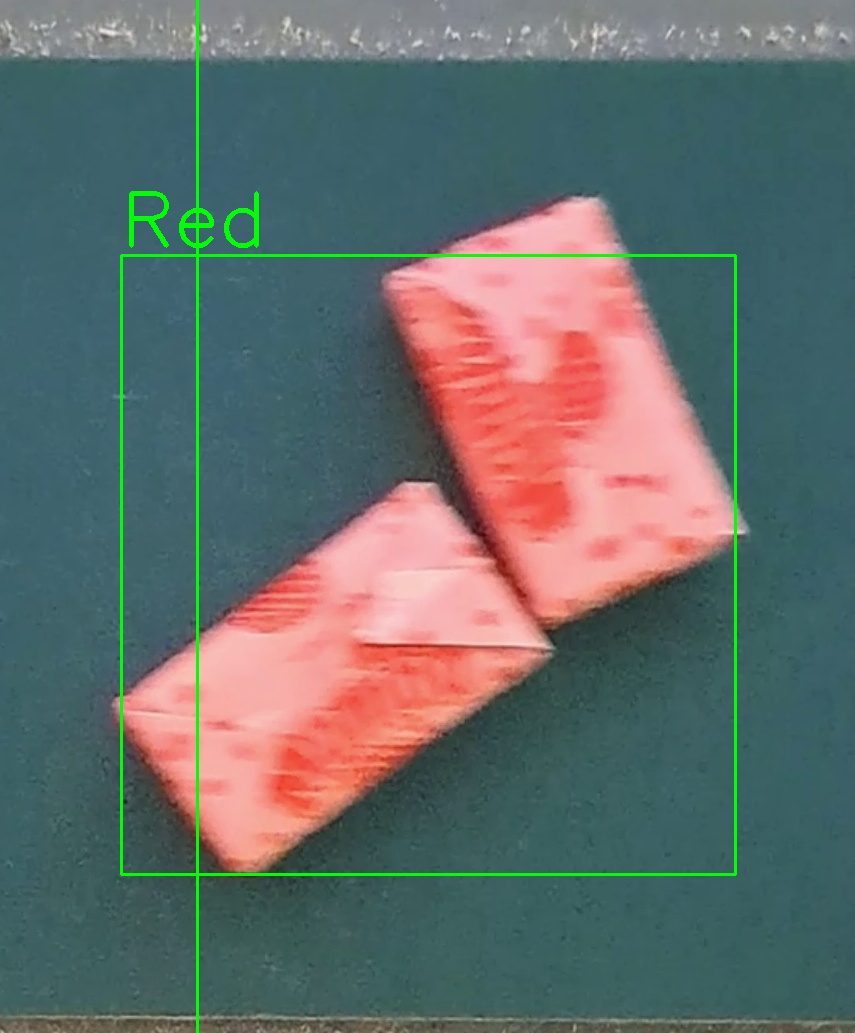
\includegraphics[height=5cm]{red.png}
\caption{Przypadek błędu metody, w którym para cukierków tego samego typu jest traktowana jako jeden cukierek}
\end{figure}
\end{center}

\section{Wnioski}
\label{Wnioski}

Projekt skoncentrował się na opracowaniu metody klasyfikacji cukierków na podstawie koloru ich opakowań. Metoda klasyfikacji osiągneła średnią skuteczność 96\% dla analizowanego nagrania przykładowego użycia. Skuteczność na tym poziomie może być wystarczająca dla takich przypadków użycia, w których stu procentowa precyzja nie jest wymagana. Jednym z takich przypadków może być weryfikacja różnorodności cukierków na taśmie produkcyjnej. W tym przypadku nie jest wymagane zliczenie dokładnej ilości cukierków danego typu, a jedynie sprawdzenie, czy cukierki są wystarczająco zróżnicowane przyjmując pewien próg różnorodności.

Perspektywy rozwoju obejmują dalsze doskonalenie algorytmu klasyfikacji, zwłaszcza w przypadku sytuacji, gdy cukierki tego samego koloru opakowania są blisko siebie. Dodatkowo, można rozważyć rozszerzenie rozwiązania na inne produkty spożywcze o podobnych wymiarach, co zwiększyłoby zakres jego zastosowania.

\section{Literatura}
\label{Literatura}
\begin{thebibliography}{9}

\bibitem{virtuslab}
\url{https://virtuslab.com/case-study/object-detection-in-real-time-streaming-recordings-and-images}

\bibitem{gfg}
\url{https://www.geeksforgeeks.org/detect-an-object-with-opencv-python/}

\bibitem{coalForeign}
\url{https://www.mdpi.com/2227-7080/11/5/114}

\bibitem{dry}
\url{https://dontrepeatyourself.org/post/color-based-object-detection-with-opencv-and-python/}

\bibitem{yt-motorcycle}
\url{https://www.youtube.com/watch?v=O3b8lVF93jU/}

\bibitem{yt-banana}
\url{https://www.youtube.com/watch?v=aFNDh5k3SjU&t=1004s/}

\bibitem{chocolates}
\url{https://blog.roboflow.com/identifying-chocolates-with-computer-vision/}

\bibitem{vending}
 \url{https://www.researchgate.net/publication/337068624_Towards_Identification_of_Packaged_Products_via_Computer_Vision_Convolutional_Neural_Networks_for_Object_Detection_and_Image_Classification_in_Retail_Environments}

\bibitem{inRange}
\url{https://docs.opencv.org/3.4/d2/de8/group__core__array.html#ga48af0ab51e36436c5d04340e036ce981}

\bibitem{findContours}
\url{https://docs.opencv.org/3.4/d3/dc0/group__imgproc__shape.html#ga17ed9f5d79ae97bd4c7cf18403e1689a}

\bibitem{retrExternal}
\url{https://docs.opencv.org/4.x/d3/dc0/group__imgproc__shape.html#gga819779b9857cc2f8601e6526a3a5bc71aa7adc6d6608609fd84650f71b954b981}

\bibitem{chainApproxSimble}
\url{https://docs.opencv.org/4.x/d3/dc0/group__imgproc__shape.html#gga4303f45752694956374734a03c54d5ffa5f2883048e654999209f88ba04c302f5}

\end{thebibliography}

\end{document}